\newsavebox\myboxa
\savebox\myboxa{%
	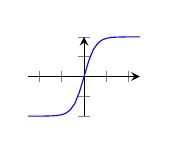
\begin{tikzpicture}
		\begin{axis}[
		  axis lines=middle,
		  width=3cm,
		  xticklabels={,,},
		  yticklabels={,,}
		]
		\addplot+[no marks] {tanh(x)};
		\end{axis}
	\end{tikzpicture}%
}

\def\layersep{3cm}
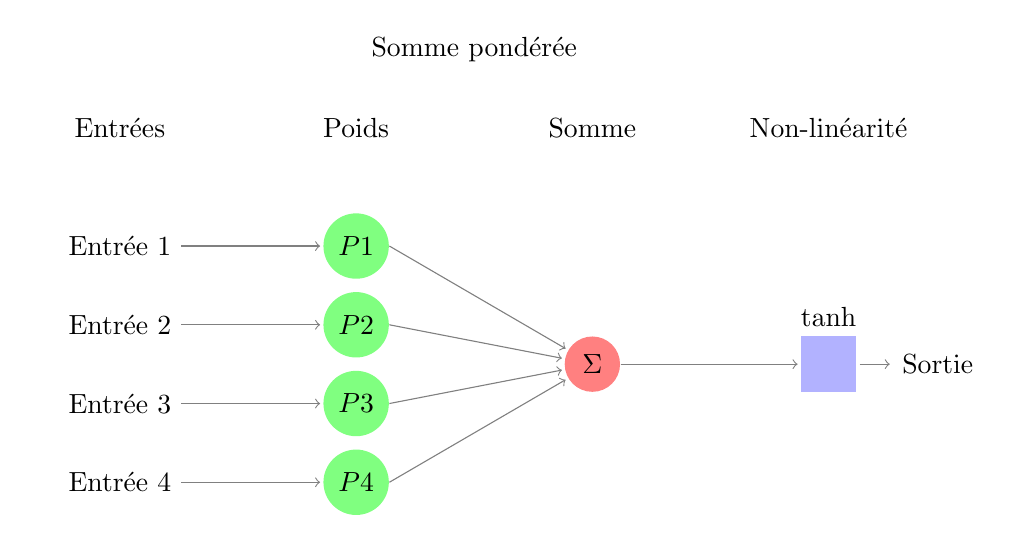
\begin{tikzpicture}[shorten >=1pt,->,draw=black!50, node distance=\layersep]
    \tikzstyle{every pin edge}=[<-,shorten <=1pt]
    \tikzstyle{input}=[rectangle];
    \tikzstyle{weight}=[circle,minimum size=20pt, fill=green!50,xshift=-1cm];
    \tikzstyle{output neuron}=[circle,minimum size=20pt, fill=red!50];
    \tikzstyle{nonlinearity}=[rectangle,minimum size=20pt, fill=blue!30];
    \tikzstyle{annot} = [text width=6em, text centered]

    % Draw the input layer nodes
    \foreach \name / \y in {1,...,4}
    % This is the same as writing \foreach \name / \y in {1/1,2/2,3/3,4/4}
        \node[input] (I-\name) at (0,-\y) {Entr\'{e}e \y};
    \foreach \name / \y in {1,...,4}
        \node[weight,right of=(I-\name)] (W-\name) at (1,-\y) {$P\name$};

    % Draw the output layer node
    \node[output neuron, right of=I-1, right of=I-2,xshift=-1cm] (Syn) at (,-2.5) {$\Sigma$};
    % Draw the output layer node
    \node[nonlinearity,pin={[pin edge={->}]right:Sortie}, right of=Syn,label=above:$\tanh$] (NL) {\usebox\myboxa};

    % Connect every node in the input layer with every node in the
    % hidden layer.
    \foreach \source in {1,...,4}
        \path (I-\source.east) edge (W-\source.west);
    \foreach \source in {1,...,4}
        \path (W-\source.east) edge (Syn);
	\path (Syn) edge (NL);

    % Annotate the layers
    \node[annot,above of=I-1, node distance=1.5cm] (hl) {Entr\'{e}es};
    \node[annot,above of=W-1, node distance=1.5cm] (pl) {Poids};
    \node[annot,above of=Syn] (sl) {Somme};
    \node[annot,above of=pl, above of=sl, node distance=.5cm,text width=12em,xshift=-1.5cm] (hl) {Somme pond\'{e}r\'{e}e};
    \node[annot,above of=NL] (hl) {Non-lin\'{e}arit\'{e}};
\end{tikzpicture}